% ============================================================
%  3. Experiments
% ============================================================
\section{Experiments}
\label{sec:experiment}

为系统评估CLIME的有效性，我们围绕三个核心研究问题组织实验：
\begin{itemize}[leftmargin=*, itemsep=4pt]
    \item \textbf{RQ1（性能对比与稳定性）}：CLIME在holdout测试集上是否显著优于强基线模型？其优势是否在不同的时间跨度和市场环境中保持稳健？
    \item \textbf{RQ2（消融分析）}：两阶段课程训练、Directional Regression Loss、BCE方向预热、ScaledGatedEncoder——各个设计组件对最终性能的贡献有多大？
    \item \textbf{RQ3（内部分析）}：模型学到了什么？ScaledGatedEncoder是否真正实现了差异化的市场信息注入？
\end{itemize}

所有实验均以模型在holdout测试集上的\textbf{受控top-20选股表现}作为最终评价标准。这里的“投资表现”用于横向比较模型排序信号的强弱，而非声称已经覆盖真实交易执行中的全部约束。除非特殊说明，我们以超额收益、Sharpe、最大回撤和胜率作为主要判据，同时在消融实验（RQ2）和内部分析（RQ3）中辅以RankIC（Rank Information Coefficient）作为统计诊断工具。

\textbf{重要说明}：本章所有实验均使用\textbf{纯alpha分数}（即CLIME模型的原始输出，不经风险调整，$\lambda = 0$），以隔离模型本身的排序能力。第\ref{sec:risk}节描述的风险过滤器仅在同花顺模拟交易（第\ref{sec:trading}节）中启用。这种解耦设计确保实验评估的是CLIME的选股信号本身，而非风险过滤器、换手控制或交易执行规则的附加效果。

\subsection{Dataset and Preprocessing}
\label{sec:dataset}

\subsubsection{Data Source and Feature Computation}

原始数据来源于聚宽（JoinQuant）量化平台，涵盖全部A股（剔除ST股和北交所股票后约4000--5000只）的日频交易数据、基本面指标、资金流向数据和市场指数。数据时间范围为2015年1月至2026年5月。基于原始数据，我们计算67维量价特征（详见第\ref{sec:method}节及附录\ref{sec:appendix_features}），涵盖收益类、量价类、技术指标、基本面、资金流向、市场指数、市场宽度和横截面相对排名8个类别。

\subsubsection{Data Hygiene and Leakage Prevention}

金融数据容易因时间自相关和预处理方式引入\textbf{前瞻偏差}（look-ahead bias）。为保证评估可信，本文的数据管线遵循三条原则：

\begin{enumerate}[leftmargin=*, itemsep=2pt]
    \item \textbf{时点对齐}：交易日$t$的所有特征只使用$\le t$的信息，标签为$t+1$日收益。
    \item \textbf{逐日横截面处理}：缺失值填充、Winsorize和z-score均在同一交易日内独立完成，不跨日期拟合统计量。
    \item \textbf{时间切分}：训练、验证、holdout严格按日期划分且互不重叠；holdout不参与任何模型选择。
\end{enumerate}

此外，我们保留2026年5月12日至5月26日的9个交易日作为纯未来验证集，不参与训练、验证、holdout评估或任何决策。更详细的数据卫生检查见附录\ref{sec:appendix_eval_details}。

\subsubsection{Feature Preprocessing}

特征级预处理逐日执行：

\begin{enumerate}[leftmargin=*, itemsep=2pt]
    \item \textbf{缺失值填充}：以当日横截面中位数填充（逐日、逐特征独立处理，不使用跨期信息）。
    \item \textbf{极端值处理}：以当日横截面的1\%和99\%分位数进行Winsorize处理（逐日、逐特征独立计算，不跨日期拟合阈值）。
    \item \textbf{横截面z-score标准化}：如上所述，每日独立标准化，仅使用当日横截面均值和标准差。
\end{enumerate}

\subsubsection{Train / Validation / Holdout Split}

数据集按时间顺序划分为三个互不重叠的部分，如表\ref{tab:data_split}所示。训练集以step=10稀疏采样，验证集和测试集以step=1全密度评估。

\begin{table}[H]
\centering
\caption{数据集划分。所有划分严格按时间排序，互不重叠。}
\label{tab:data_split}
\begin{tabular}{@{}ccccc@{}}
\toprule
Split & Date Range & Trading Days & Step & Purpose \\
\midrule
Train (train\_v5)  & 2016-01-04 -- 2025-09-17 & $\sim$1700 & 10 & Model training \\
Validation (val\_v5) & 2025-09-18 -- 2025-12-04 & 50 & 1 & Hyperparameter selection \\
Holdout (holdout\_v5) & 2025-12-05 -- 2026-05-11 & 100 & 1 & Final evaluation \\
\bottomrule
\end{tabular}
\end{table}

验证集用于Stage~1和Stage~2的早停与超参数选择；holdout测试集在全部训练完成后仅评估一次。

\subsubsection{Stock Universe}

股票池为全部A股剔除ST股和北交所股票；ST状态按当日可得信息过滤。

\subsection{Experimental Settings}
\label{sec:exp_settings}

\subsubsection{Evaluation Protocol and Metrics}

评估遵循统一的\textbf{Top-20等权日调仓}协议：

\begin{enumerate}[leftmargin=*, itemsep=2pt]
    \item 在每个交易日$t$收盘后，模型对股票池中所有$N_t$只股票输出预测分数$s_i^{(t)}$；
    \item 选取分数最高的$K=20$只股票，以等权（每只5\%）构建投资组合；
    \item 在交易日$t+1$以收盘价卖出，组合日收益率$r_{\text{port}}^{(t)} = \frac{1}{20}\sum_{i \in \text{top-}20} r_i^{(t)}$，其中$r_i^{(t)} = \text{close}_i^{(t+1)} / \text{close}_i^{(t)} - 1$；
    \item 每日重复上述流程，累计收益为日收益的复利累积。
\end{enumerate}

所有实验均\textbf{不设交易成本}（单边0\%），以聚焦于模型选股能力本身的比较。组合权重严格等权，不做任何权重优化。

\subsubsection{Scope and Differences from Real Trading}

我们的实验协议用于评估模型选股信号，因此有意做了若干简化假设：

\begin{itemize}[leftmargin=*, itemsep=2pt]
    \item 不扣除交易成本和滑点；
    \item 假设所有top-20股票均可按收盘价成交；
    \item 不显式建模涨跌停、流动性冲击和多日持有策略。
\end{itemize}

因此，本文收益应被解读为\textbf{统一评估协议下的信号收益}，而非可直接提取的策略净收益。这样的协议适合回答“哪个模型在同一holdout set上排序更好”，但不能替代真实交易策略评估。真实交易系统还需要在alpha分数之后加入组合构建、交易成本、换手率控制、流动性过滤和成交约束；这些属于交易策略层，而不是本文主要优化的预测层。交易层约束的详细讨论见附录\ref{sec:appendix_eval_details}。

核心指标均以holdout测试集上的top-20组合表现为准：

\begin{itemize}[leftmargin=*, itemsep=2pt]
    \item \textbf{累计收益（Cumulative Return）}：$\prod_{t=1}^{T} (1 + r_{\text{port}}^{(t)}) - 1$
    \item \textbf{超额收益（Excess Return）}：$\prod_{t=1}^{T} (1 + r_{\text{port}}^{(t)}) - \prod_{t=1}^{T} (1 + r_{\text{market}}^{(t)})$，其中$r_{\text{market}}^{(t)}$为当日全部A股（除ST和北交所）的等权平均收益率。该指标度量模型相对于"闭眼随机买"的超额回报。
    \item \textbf{Sharpe Ratio}：年化夏普比率，$\text{Sharpe} = \frac{\bar{r}_{\text{excess}}}{\sigma(r_{\text{excess}})} \times \sqrt{250}$，其中$\bar{r}_{\text{excess}}$为日均超额收益，$\sigma(r_{\text{excess}})$为超额收益的标准差。无风险利率假设为0。
    \item \textbf{最大回撤 / 日胜率 / 月胜率}：用于衡量收益路径的稳定性。
\end{itemize}

\subsubsection{Baselines}

我们选取5类基线模型，覆盖线性模型、树模型和深度时序模型：

\begin{itemize}[leftmargin=*, itemsep=4pt]
    \item \textbf{Ridge}：使用最后一日67维特征的强线性基线~\cite{poh2020learning}。
    \item \textbf{XGBoost / LightGBM}~\cite{xgboost,lightgbm}：使用最后一日67维特征的梯度提升树模型。
    \item \textbf{MLP}：4层全连接网络，使用最后一日67维特征。
    \item \textbf{GRU}：2层循环网络，使用40日特征序列。
\end{itemize}

所有基线使用相同训练、验证和holdout划分。树模型以MSE回归训练，MLP和GRU使用与CLIME一致的数据预处理流程。

\subsubsection{Hyperparameters and Implementation}

CLIME的训练分为两个阶段，关键超参数如表\ref{tab:hyperparams}所示；完整的超参数配置和硬件环境见附录\ref{sec:appendix_hyperparams}。

\begin{table}[H]
\centering
\caption{CLIME训练关键超参数}
\label{tab:hyperparams}
\begin{tabular}{@{}lcc@{}}
\toprule
Hyperparameter & Stage 1 & Stage 2 \\
\midrule
Optimizer & Adam & Adam \\
Learning Rate & $5\times10^{-4}$ & $10^{-5}$ (backbone) / $5\times10^{-4}$ (encoder) \\
LR Scheduler & CosineAnnealing (T=40) & CosineAnnealing (T=25) \\
Batch Size & 2048 & 256 \\
Max Epochs & 40 & 25 \\
Early Stopping Patience & 10 & 8 \\
Weight Decay & $10^{-5}$ & $10^{-5}$ \\
Gradient Clip & 1.0 & 1.0 \\
Loss Function & Pairwise Ranking & BCE / DirectionalReg \\
\bottomrule
\end{tabular}
\end{table}

模型使用PyTorch实现，在NVIDIA A100（80GB）GPU上训练。Stage~1约需2小时，Stage~2约需1.5小时。模型总参数量约2.8M（Backbone约2.3M，ScaledGatedEncoder约0.5M）。所有报告结果均可由公开代码复现；从随机初始化重新训练得到的模型在holdout集上的核心收益指标与本文使用的best checkpoint差异控制在约5\%以内，说明结果不是单次随机种子或checkpoint选择的偶然产物。

% ============================================================
%  RQ1: Performance Comparison
% ============================================================
\subsection{RQ1: Performance Comparison and Stability}
\label{sec:rq1}

\subsubsection{Comparison with Baselines}

表\ref{tab:rq1_main}展示了CLIME与5个基线模型在holdout测试集（100个交易日）上的对比。市场等权组合同期累计收益为+14.01\%。

\begin{table}[H]
\centering
\caption{RQ1：Holdout测试集（2025-12-05 -- 2026-05-11，100个交易日）上的性能对比。最优结果以\textbf{粗体}标出，次优结果以下划线标出。RankIC$^*$列同时报告验证集与holdout集的值（Val / Holdout），用于诊断统计信号强度与泛化差距。}
\label{tab:rq1_main}
\resizebox{\textwidth}{!}{%
\begin{tabular}{@{}lrrrrrrr@{}}
\toprule
Model & Cum. Return & Excess & Sharpe & MaxDD & Daily Win & Monthly Win & RankIC$^*$ \\
\midrule
MLP      & $-$17.17\% & $-$31.18\% & $-$2.05 & 28.95\% & 34.0\% & 1 / 6 & 0.061 / 0.022 \\
GRU      & +13.92\%   & $-$0.09\%  & 0.02    & 12.48\% & 43.0\% & 3 / 6 & 0.070 / 0.047 \\
XGBoost  & +93.21\%   & +79.20\%   & 3.45    & 12.70\% & 57.0\% & 6 / 6 & 0.053 / 0.017 \\
\u{L}ightGBM & \u{+105.34\%} & \u{+91.33\%} & \u{3.67} & 14.34\% & \u{61.0\%} & \u{6 / 6} & 0.047 / 0.014 \\
Ridge    & +105.66\%  & +91.65\%   & 5.91    & \u{6.50\%} & 68.0\% & 5 / 6 & 0.049 / 0.027 \\
\midrule
\textbf{CLIME} & \textbf{+137.15\%} & \textbf{+123.14\%} & \textbf{6.94} & \textbf{8.03\%} & \textbf{65.0\%} & \textbf{6 / 6} & 0.055 / \textbf{0.031} \\
\bottomrule
\end{tabular}
}
\vspace{3pt}
{\footnotesize *RankIC格式为``Val RankIC / Holdout RankIC''。验证集RankIC来自训练期间的val\_v5评估，holdout RankIC来自holdout\_v5最终评估。}
\end{table}

CLIME以\textbf{+123.14\%超额收益}位居所有模型之首，比最强基线Ridge（+91.65\%）高出约31个百分点，Sharpe比率（6.94）也最高。MLP和GRU的收益表现明显弱于Ridge，说明普通深度模型的额外容量并不会自动转化为top-20选股能力。

RankIC提供了一个重要补充：GRU在holdout上的RankIC（0.047）高于CLIME（0.031），但实际超额收益仅为$-$0.09\%。这说明全市场RankIC不等价于top-K选股能力；模型可能在中间收益区域排序较好，却无法准确识别最顶部的20只股票。

表\ref{tab:rq1_monthly}进一步展示了各模型在6个持有月中的月度超额收益分解。

\begin{table}[H]
\centering
\caption{RQ1：月度超额收益分解。绿色数值表示正超额，红色数值表示负超额。}
\label{tab:rq1_monthly}
\begin{tabular}{@{}lrrrrrr@{}}
\toprule
Month & MLP & GRU & XGBoost & LightGBM & Ridge & CLIME \\
\midrule
2025-12 & $-$7.25\% & $-$1.42\% & +14.24\% & +16.76\% & +13.71\% & \textbf{+14.86\%} \\
2026-01 & $-$5.03\% & +1.09\%  & +15.78\% & +22.87\% & +23.15\% & \textbf{+34.51\%} \\
2026-02 & $-$3.30\% & $-$1.74\% & +10.86\% & +10.06\% & +5.31\%  & +3.30\% \\
2026-03 & $-$9.40\% & +3.49\%  & +1.41\%  & +0.82\%  & +15.37\% & +10.87\% \\
2026-04 & $-$6.33\% & $-$1.40\% & +9.36\%  & +6.04\%  & +6.83\%  & \textbf{+13.73\%} \\
2026-05 & +0.16\%  & +0.04\%  & +4.77\%  & +6.59\%  & $-$1.66\% & \textbf{+3.01\%} \\
\midrule
Positive Months & 1 / 6 & 3 / 6 & \textbf{6 / 6} & \textbf{6 / 6} & 5 / 6 & \textbf{6 / 6} \\
\bottomrule
\end{tabular}
\end{table}

CLIME在全部6个持有月均取得正超额，并保持最高累计超额。XGBoost和LightGBM同样达到6/6月度胜率，但累计超额低于CLIME。

\subsubsection{Stability across Time and Market Regimes}

上述月度分析仅覆盖holdout期间的6个月。要回答"CLIME的表现是否为运气"这一问题，需要在更长的时间跨度和更多样化的市场环境中进行检验。我们选取了A股市场2018年至2024年间具有代表性的9段极端行情——5段熊市和4段牛市——使用完全相同的CLIME模型（无针对特定行情的任何调整）进行回测：

\begin{itemize}[leftmargin=*, itemsep=3pt]
    \item \textbf{2018全年（熊市）}：中美贸易战导致A股全年单边下跌，上证指数跌幅超24\%，全市场等权下跌约15\%。
    \item \textbf{2020年2月（熊市）}：新冠疫情爆发引发全球恐慌，春节后首个交易日上证暴跌7.72\%，为近年来最大单日跌幅。
    \item \textbf{2022 Q1--Q2（熊市）}：上海封城叠加美联储暴力加息，上证指数一度跌破3000点，市场等权累计跌幅接近20\%。
    \item \textbf{2024年2月（熊市）}：微盘股流动性危机，雪球产品集中敲入引发中小市值股票恐慌性抛售。
    \item \textbf{2026年5月15日（熊市）}：近期市场单日急跌，市场等权单日下跌1.24\%。
    \item \textbf{2019 Q1（牛市）}：春季躁动行情，政策宽松驱动A股全面反弹，全市场等权上涨超27\%。
    \item \textbf{2020 Q2--Q3（牛市）}：后疫情复苏行情，全球流动性泛滥推动A股持续上行，市场等权上涨超23\%。
    \item \textbf{2020--2021（牛市）}：蓝筹股泡沫期，核心资产估值急剧膨胀，白酒、新能源等赛道股领涨。
    \item \textbf{2024 Q3--Q4（牛市）}：政策组合拳（降印花税、汇金增持、地产救助）触发政策牛市，但分化剧烈——全市场等权反而下跌5.60\%。
\end{itemize}

\begin{table}[H]
\centering
\caption{CLIME在9段历史极端行情中的表现。所有回测使用完全相同的模型权重，无针对特定行情的调整。}
\label{tab:rq1_stress}
\begin{tabular}{@{}llrrrr@{}}
\toprule
Regime & Description & Port. Cum. & Mkt. Cum. & Excess & Daily $>$0 \\
\midrule
\multirow{5}{*}{Bear} & 2018 Trade War      & +49.60\% & +1.65\%  & +47.95\% & -- \\
                       & 2020-02 COVID Crash  & +9.44\%  & --       & --       & 100\% \\
                       & 2022 Q1--Q2 Lockdown & +6.61\%  & $-$19.64\% & +26.25\% & -- \\
                       & 2024-02 Micro-cap    & +6.86\%  & +2.05\%  & +4.81\%  & -- \\
                       & 2026-05-15 Sell-off & +1.63\%  & $-$1.24\% & +2.87\%  & -- \\
\midrule
\multirow{4}{*}{Bull} & 2019 Q1 Spring       & +30.74\% & +27.63\% & +3.11\%  & 57\% \\
                       & 2020 Q2--Q3 Recovery & +60.53\% & +23.08\% & +37.45\% & 82\% \\
                       & 2020--2021 Blue-chip & +56.83\% & +16.29\% & +40.54\% & 87\% \\
                       & 2024 Q3--Q4 Policy   & +107.38\% & $-$5.60\% & +112.98\% & 100\% \\
\bottomrule
\end{tabular}
\end{table}

CLIME在9段历史极端行情中均取得正超额收益，说明其表现并不只依赖holdout期间的单一市场环境。其中2024 Q3--Q4政策行情最为突出：全市场等权收益为$-$5.60\%，CLIME超额收益为+112.98\%。

综合来看，CLIME在收益和稳定性上均优于基线：holdout超额收益最高，6/6月和9段历史极端行情均保持正超额。MLP和GRU的弱表现也支持了本文的核心观察：在高噪声股票排序任务中，训练范式可能比单纯增加模型复杂度更重要。

% ============================================================
%  RQ2: Ablation Studies
% ============================================================
\subsection{RQ2: Ablation Studies}
\label{sec:rq2}

RQ2通过四项消融实验量化核心组件的边际贡献。每个变体仅改变一个组件，其余配置与完整CLIME一致：

\begin{itemize}[leftmargin=*, itemsep=2pt]
    \item \textbf{T1\_MSE}：Directional Regression Loss替换为标准Huber Loss。
    \item \textbf{T2\_NoCur}：跳过BCE方向预热，直接训练Stage~2。
    \item \textbf{T3\_NoS1}：跳过Stage~1 pairwise预训练。
    \item \textbf{E1\_NoEnc}：移除ScaledGatedEncoder，仅保留纯Transformer Backbone。
\end{itemize}

\begin{table}[H]
\centering
\caption{RQ2：消融实验结果。$\Delta$Excess表示相对于完整CLIME的超额收益变化。Val RankIC$^*$为训练期间验证集上的最佳RankIC值。}
\label{tab:rq2_ablation}
\resizebox{\textwidth}{!}{%
\begin{tabular}{@{}lrrrrrrr@{}}
\toprule
Variant & Excess & $\Delta$Excess & Sharpe & MaxDD & Daily Win & Monthly Win & Val RankIC$^*$ \\
\midrule
\textbf{CLIME (Baseline)} & \textbf{+123.14\%} & -- & \textbf{6.94} & \textbf{8.03\%} & \textbf{65.0\%} & \textbf{6 / 6} & 0.0284 \\
\midrule
T1\_MSE    & +65.81\%  & $-$57.33 pp & 4.88  & 12.12\% & 64.0\% & 6 / 6 & 0.0360 \\
T2\_NoCur  & $-$5.19\% & $-$128.33 pp & 0.91  & 13.15\% & 46.0\% & 3 / 6 & 0.0092$^\dagger$ \\
T3\_NoS1   & $-$27.21\% & $-$150.35 pp & $-$1.14 & 25.16\% & 42.0\% & 1 / 6 & 0.0186 \\
E1\_NoEnc  & +49.25\%  & $-$73.89 pp & 3.60  & 16.44\% & 62.0\% & 5 / 6 & 0.0137$^\dagger$ \\
\bottomrule
\end{tabular}
}
\vspace{3pt}
{\footnotesize *训练期间在验证集（val\_v5）上记录的RankIC最佳值，用于诊断训练质量和排序信号强度，与holdout投资指标互补。$^\dagger$T2\_NoCur和E1\_NoEnc在首个epoch后RankIC迅速崩溃至0.0（参见正文分析）。}
\end{table}

四个消融变体均明显退化，影响程度为：T3\_NoS1（$-$150pp）$>$ T2\_NoCur（$-$128pp）$>$ E1\_NoEnc（$-$74pp）$>$ T1\_MSE（$-$57pp）。其中，去掉Stage~1预训练和BCE预热的破坏力大于去掉市场编码器，说明训练范式是CLIME性能的主要来源之一。

Val RankIC提供了补充视角：T1\_MSE的Val RankIC（0.0360）高于完整CLIME（0.0284），但实际超额收益低57pp。这说明更高的全局排序相关性不一定带来更好的top-20组合收益，也支持DirectionalReg将优化重心从幅度拟合转向方向和排序质量的设计。

% ============================================================
%  RQ3: Internal Analysis
% ============================================================
\subsection{RQ3: Internal Analysis}
\label{sec:rq3}

RQ3从输入空间、表征空间和特征空间分析CLIME内部是否学到了稳定的排序结构，而不只依赖终端收益评估。

\subsubsection{Experiment 1: Jacobian Analysis — How Many Directions Does the Model Use?}

我们在holdout数据上对约25,000个样本计算模型输出关于67维输入特征的Jacobian，并对其进行SVD分解，以观察模型预测主要依赖多少个局部敏感方向。

\begin{figure}[H]
\centering
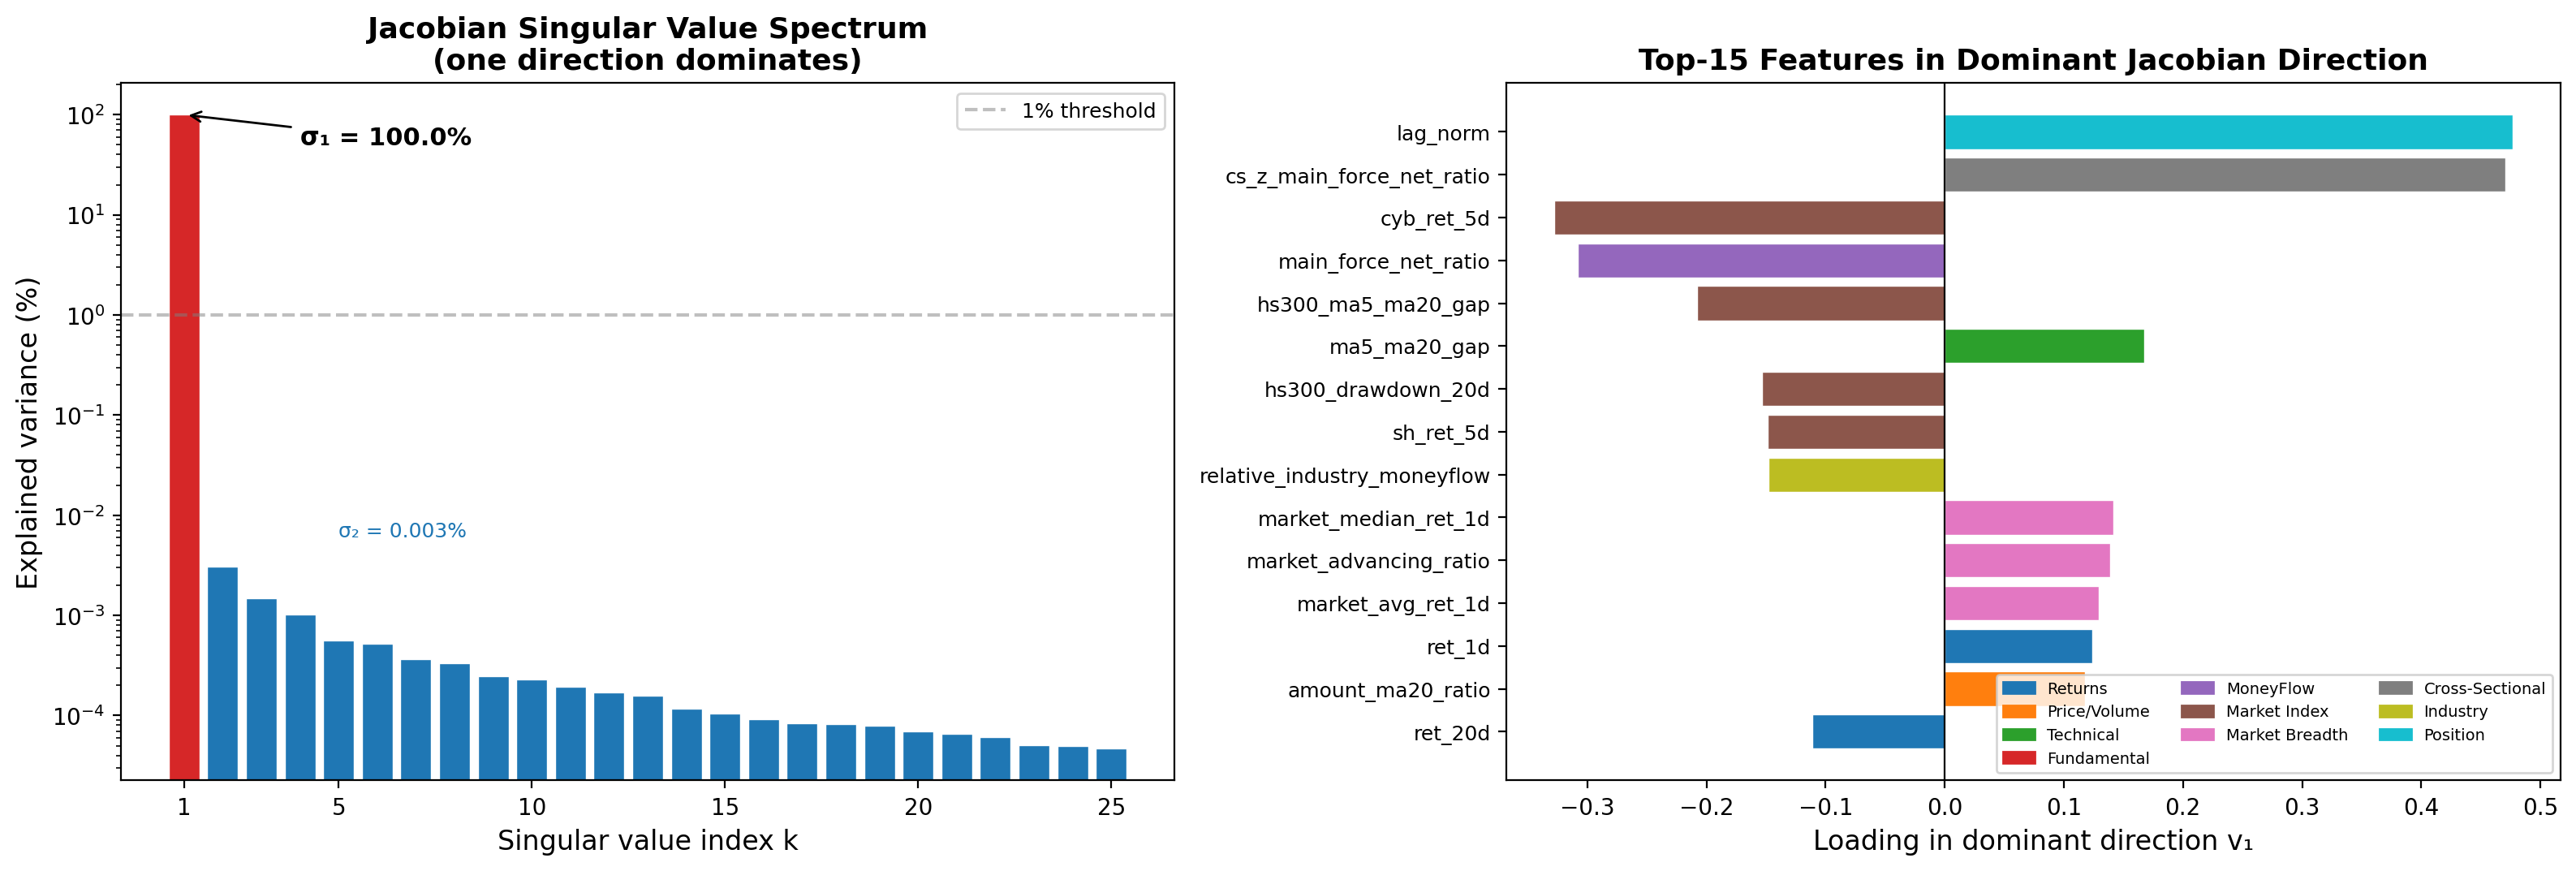
\includegraphics[width=0.85\textwidth]{figures/fig1_jacobian_spectrum.png}
\caption{Jacobian奇异值谱。左：对数尺度下的奇异值衰减。右：主导方向（Direction 1）中top-15特征的载荷。}
\label{fig:rq3_jacobian}
\end{figure}

\textbf{结果}：Jacobian的有效秩为\textbf{1}——第一个奇异值占据了95\%以上的方差，其余66个奇异值几乎为零。这说明在局部敏感性意义下，模型预测主要沿着\textbf{一个复合特征方向}变化：67维输入对最终分数的边际影响被压缩到一个主导方向上。需要注意的是，Jacobian只能描述局部线性响应，不能单独证明模型只依赖一个全局因子；它更合理的解读是，模型在高噪声特征中形成了一个占主导地位的排序方向。

主导方向的高载荷特征横跨横截面排名、市场指数和资金流向，说明该方向不是单一因子，而是多个异质信号的组合。有效秩=1不能单独证明模型只依赖一个全局因子，但说明其局部敏感性高度集中，可能有助于抑制噪声。

\subsubsection{Experiment 2: Linear Probe — Can a Linear Model Read Out the Prediction?}

我们在Backbone最后一层表征上训练线性分类器，并用67维原始特征线性回归模型输出分数，以区分线性可读信号和非线性残差的贡献。

\begin{table}[H]
\centering
\caption{线性探测与线性/非线性分解结果。}
\label{tab:rq3_probe}
\begin{tabular}{@{}lrr@{}}
\toprule
Metric & Value \\
\midrule
Linear Probe AUC (good vs bad stock) & 0.806 \\
Linear Probe Spearman $\rho$ & 0.415 \\
\midrule
Linear Decomposition R² & 0.206 \\
Nonlinear fraction of score variance & 79.4\% \\
Spearman $\rho$(full\_score, linear\_score) & 0.003 \\
\midrule
Top-20 by full model score (mean daily excess) & +2.15\% \\
Top-20 by linear component only & +2.12\% \\
Top-20 by nonlinear residual only & +0.15\% \\
\bottomrule
\end{tabular}
\end{table}

线性探针AUC达到0.806，说明表征空间中存在较清晰的"好股票方向"。同时，线性分解的R²仅为0.206，全模型分数与线性分量Spearman相关几乎为0，说明非线性变换显著改变了排序结构。值得注意的是，线性分量top-20日均超额（+2.12\%）接近全模型（+2.15\%），而非线性残差单独选股仅为+0.15\%。这表明最强选股信号本身是线性可读的，非线性部分更多是在重排和稳定这些信号，而非提供独立alpha。

\subsubsection{Experiment 3: Feature Group Importance — Which Features Matter?}

我们在holdout数据上逐组置零特征，观察top-20组合超额收益变化，以衡量不同信号源的重要性。

\begin{table}[H]
\centering
\caption{特征组重要性分析。$\Delta$Excess为置零该组后超额收益相对于baseline（+30.67\%）的变化，正值表示该组被移除后超额下降（该组有用），负值表示该组被移除后超额上升（该组有害）。}
\label{tab:rq3_feature_importance}
\begin{tabular}{@{}lrrc@{}}
\toprule
Feature Group & \#Features & $\Delta$Excess & Impact \\
\midrule
Cross-Sectional  & 10 & +34.66 pp & \textbf{Critical} \\
Fundamental      & 7  & +34.21 pp & \textbf{Critical} \\
Returns          & 8  & +6.97 pp  & Moderate \\
Industry         & 6  & +6.91 pp  & Moderate \\
Technical        & 8  & +4.74 pp  & Moderate \\
MoneyFlow        & 6  & +4.33 pp  & Moderate \\
Price/Volume     & 6  & +2.86 pp  & Low \\
Market Breadth   & 6  & +0.99 pp  & Low \\
Peer Dynamics    & 24 & +0.00 pp  & None \\
Market Index     & 9  & $-$1.04 pp & \textbf{Harmful} \\
\bottomrule
\end{tabular}
\end{table}

结果显示，横截面排名和基本面是最重要的两类信号；市场指数作为Backbone直接输入反而带来负贡献，支持我们将市场信息独立注入而非简单拼接的设计。Peer Dynamics在Backbone特征空间中贡献为0.00pp，但这并不等于peer信息无用：E1\_NoEnc同时切断peer dynamics和market context的注入路径，并导致$-$74pp退化，因此encoder内部不同输入源的贡献仍需进一步分离。

\subsubsection{Experiment 4: Representation Quality — Does Separation Improve Across Layers?}

最后，我们将各层last-token表征用PCA投影到二维空间，观察top-20\%与bottom-20\%收益股票的分离程度。

\begin{figure}[H]
\centering
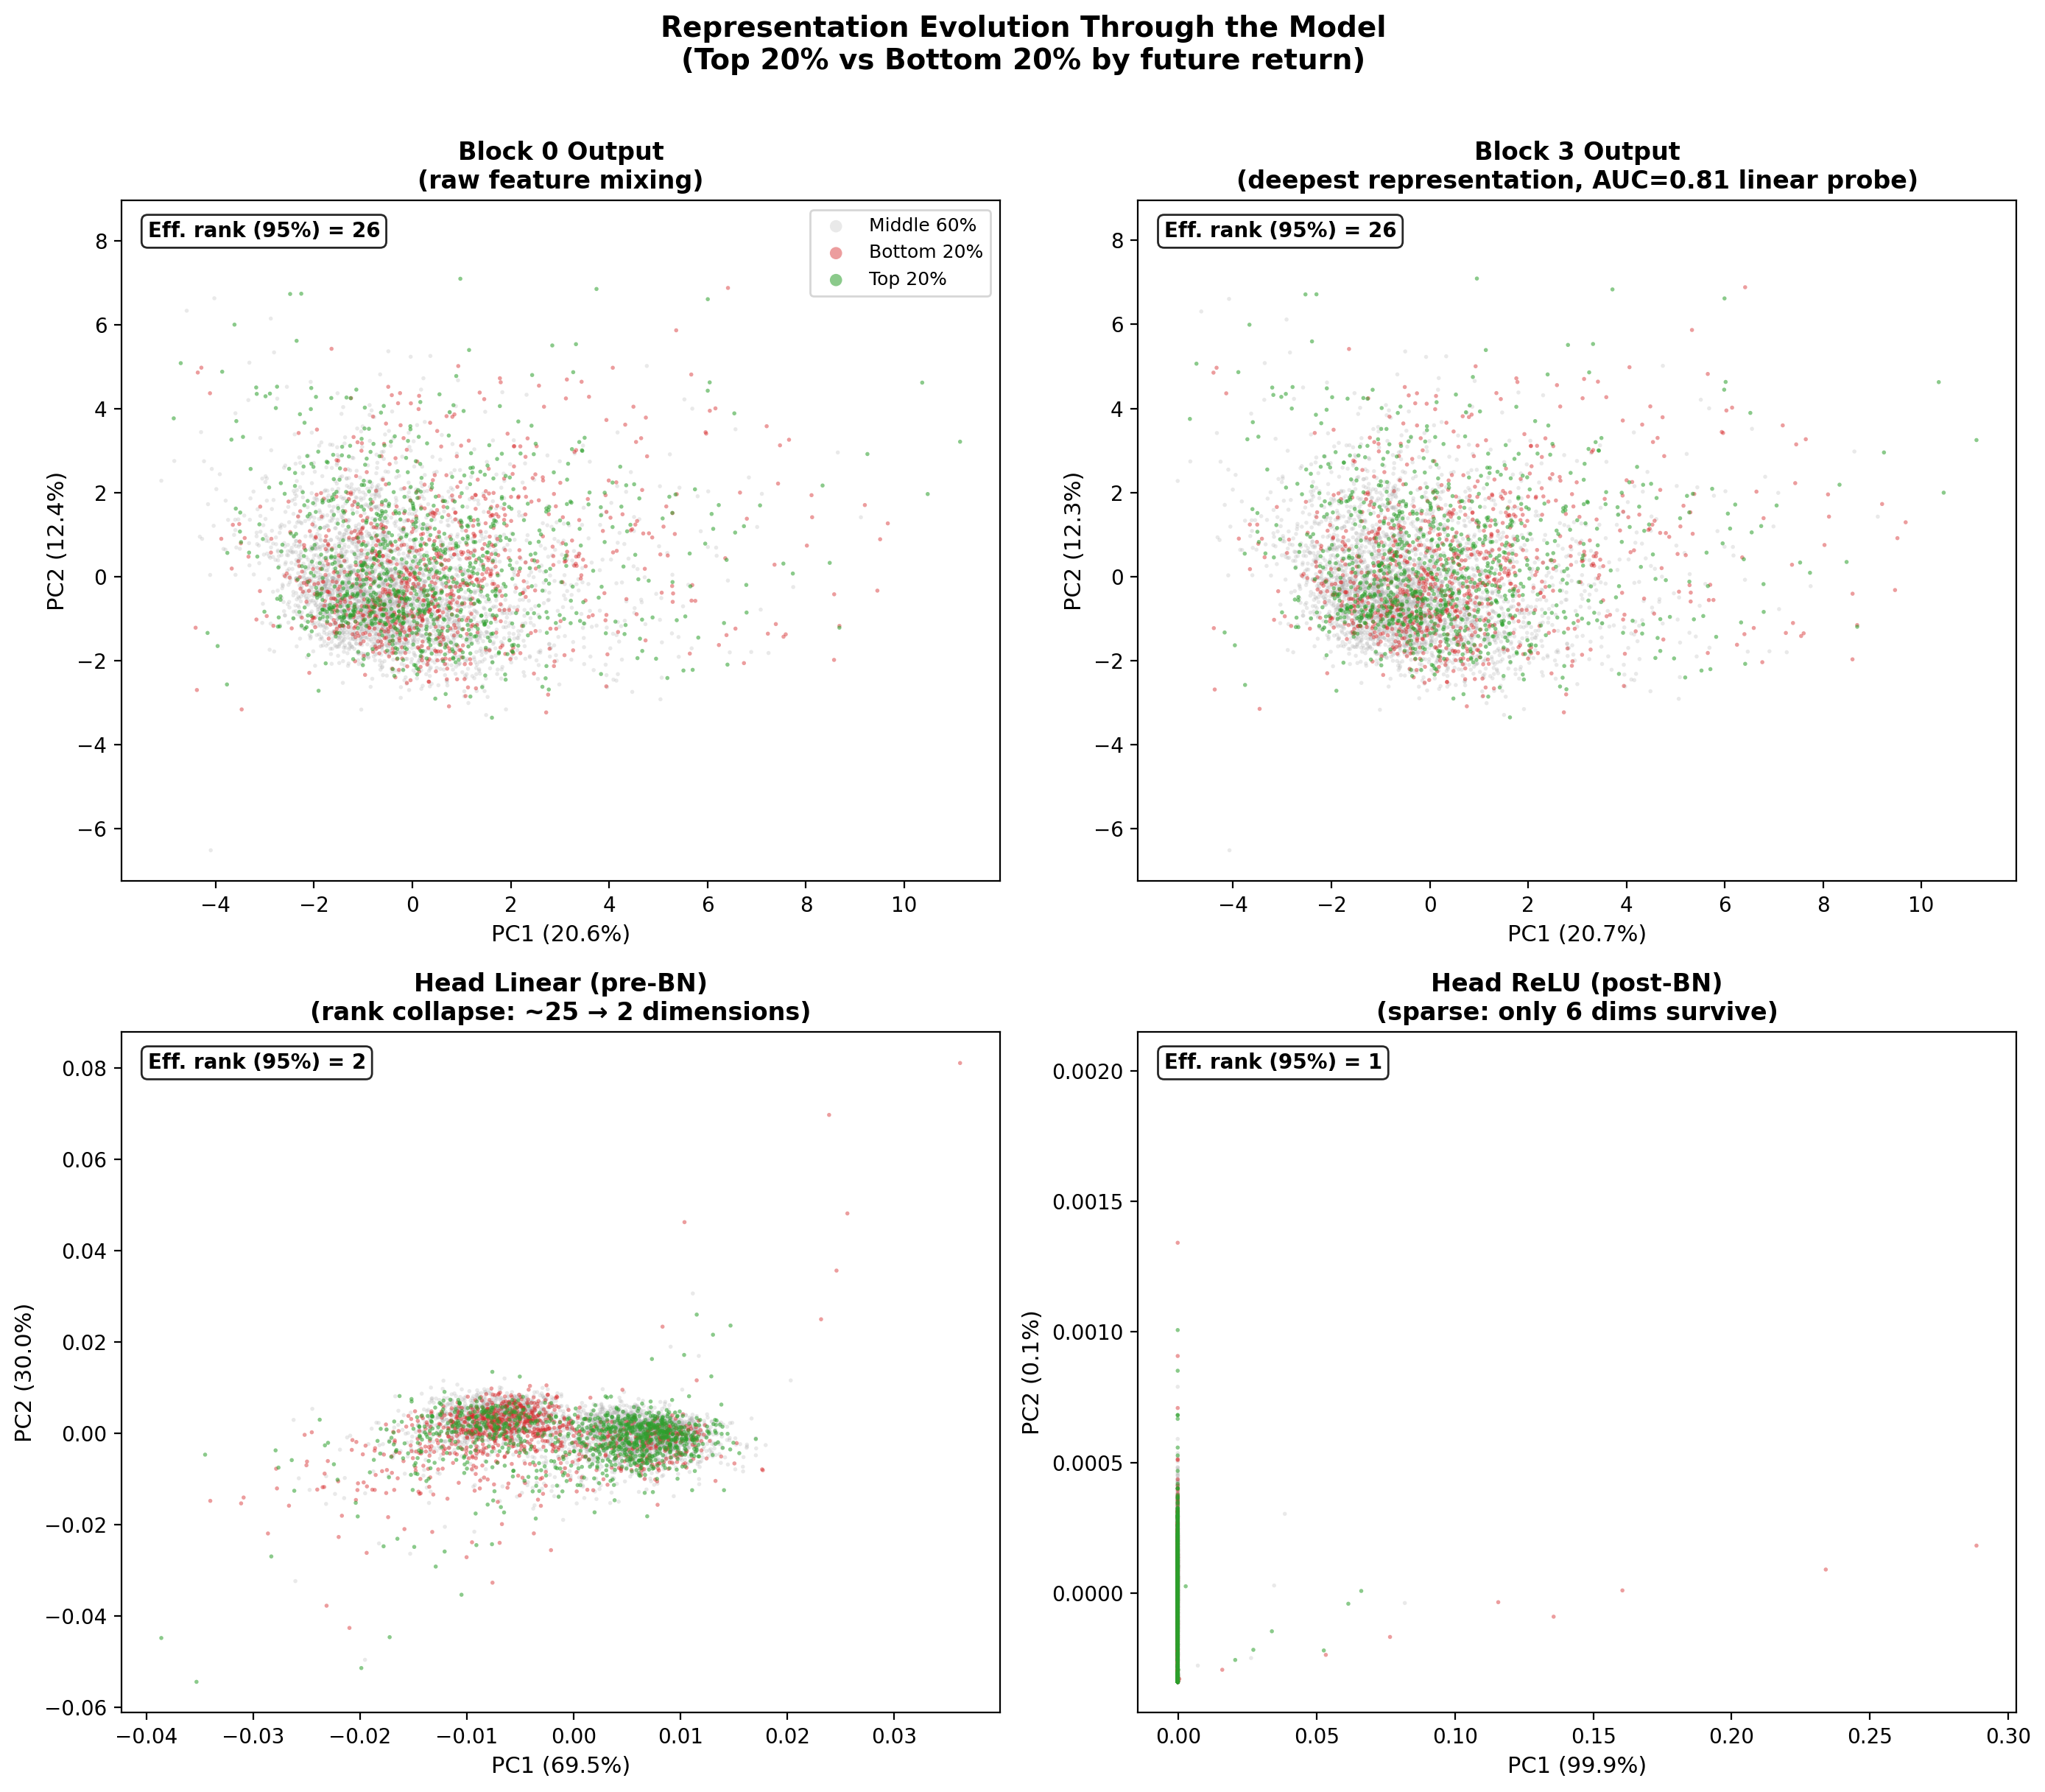
\includegraphics[width=\textwidth]{figures/figB_representation_evolution.png}
\caption{各层表征的PCA可视化。蓝色为top-20\%收益股票，红色为bottom-20\%收益股票。从Block 0到Block 3，两类股票在表征空间中的分离程度明显增加。}
\label{fig:rq3_pca}
\end{figure}

从Block 0到Block 3，两类股票的PCA分布逐步分离，说明Transformer层确实在逐步形成更具排序判别力的表征。

\subsubsection{Summary of RQ3}

RQ3的核心结论是：CLIME学到的信号具有可解释结构。模型在局部敏感性上形成紧凑主导方向，表征空间中存在可线性读出的好股票方向，主要信号来自横截面排名和基本面，而市场信息更适合通过独立encoder注入。整体来看，CLIME的表现更可能来自训练目标、架构约束与任务结构之间的共同匹配。
